%
% Risch-Algorithmus für exponentielle Erweiterungen
%
\subsection{Risch-Algorithmus für exponentielle Erweiterungen
\label{buch:intalg:risch:exponentiell}}
Abschnitt~\ref{buch:intalg:risch:logarithmisch} hat für den Fall einer
logarithmischen Erweiterung die Lücken in der allgemeinen Beschreibung
des Algorithmus in Abschnitt~\ref{buch:intalg:risch:uebersicht} gefüllt.
In diesem Abschnitt soll das Gleiche für eine exponentielle Erweiterung
getan werden.
Sei im Folgenden also $\vartheta=e^u$ ein Logarithmus eines Elements
$u\in F$.
Sie ist charakterisiert durch $D\vartheta = \vartheta\cdot Du$.

%
% Die Methode von Hermite
%
\subsubsection{Die Methode von Hermite}
In der Methode von Hermite wird benötigt, dass $b(\vartheta)$ und
$Db(\vartheta)$ teilerfremd sind.
Da $b(\vartheta)$ quadratfrei ist, sind $b(\vartheta)$ und $b'(\vartheta)$
teilerfremd.

\begin{lemma}
\label{buch:intalg:risch:exp:lemma:bDb}
Sei $b(\vartheta)\in F[\vartheta]$ ein quadratfreies Polynom.
Dann sind $b(\vartheta)$ und $Db(\vartheta)$ genau dann teilerfremd,
wenn $\vartheta$ kein Teiler von $b(\vartheta)$ ist.
\end{lemma}

\begin{proof}
Wie im Beweis von Lemma~\ref{buch:intalg:risch:log:lemma:bDb} verwenden
wir eine Faktorisierung
\[
b(\vartheta) = \prod_{i=1}^m (\vartheta-\beta_i)
\]
mit der Ableitung
\[
Db(\vartheta)
=
\sum_{k=1}^m D(\vartheta-\beta_i)\prod_{i\ne k} (\vartheta-\beta_i).
\]
Sei wieder $\vartheta-\beta_j$ ein gemeinsamer Teiler von $b(\vartheta)$
und $Db(\vartheta)$.
Dann folgt wie im Beweis von Lemma~\ref{buch:intalg:risch:log:lemma:bDb},
dass $\vartheta-\beta_j$ ein Teiler von $D(\vartheta-\beta_j)$ sein muss.
Nach dem Satz~\ref{buch:intalg:liouville:polynome:satz:logarithmisch} ist
$(\vartheta-\beta_j)\mid (D\vartheta-D\beta_j)$ genau dann, wenn der Teiler ein
Monom ist, wenn also $\beta_j=0$ und damit $\vartheta$ ein Teiler von
$b(\vartheta)$ ist.
\end{proof}

Das Lemma zeigt also, dass die Teilerfremdheit von $b(\vartheta)$ und
$Db(\vartheta)$ genau dann folgt, wenn $b(\vartheta)$ nicht durch
$\vartheta$ teilbar ist.
Schliesst man Faktoren $\vartheta$ im Nenner aus, kann die Methode von
Hermite durchgeführt werden und die Stammfunktion kann mit der Methode
von Rothstein-Trager gefunden werden.

%
% Erweiterte Polynome
%
\subsubsection{Erweiterte Polynome}
Die Diskussion der Methode von Hermite für exponentielle Erweiterungen
hat gezeigt, dass der Faktor $\vartheta$ im Nenner separat behandelt
werden muss.
Ein Faktor $\vartheta$ ist aber sehr leicht am Verschwinden des
Terms vom Grad 0 in einem Polynom erkennbar, so dass die Faktoren $\vartheta$
in der Faktorisierung
\[
q(\vartheta)
=
\vartheta^l \cdot b_1(\vartheta) b_2(\vartheta)^2 \cdots b_m(\vartheta)^m
\]
des Nenners als separate Faktoren behandelt werden können.
Die Faktoren $b_k(\vartheta)$ sind quadratfrei und nicht durch $\vartheta$
teilbar.

Die Partialbruchzerlegung von $r(\vartheta)/q(\vartheta)$ hat dann die
Form
\begin{align}
\frac{r(\vartheta)}{b(\vartheta)}
&=
\sum_{i=1}^l \frac{a_i}{\vartheta^i}
+
\sum_{i=1}^m
\sum_{k=1}^{\deg b_i(\vartheta)}
\frac{a_{ik}(\vartheta)}{b_i(\vartheta)^k}
\label{buch:intalg:risch:exp:eqn:partbruch}
\end{align}
mit $a_i\in F$ und $a_{ik}\in F[\vartheta]$.
Die zweite Summe in \eqref{buch:intalg:risch:exp:eqn:partbruch}
enthält nur Terme, die den Faktor $\vartheta$ im 
Nenner nicht enthalten und daher mit der Methode von Hermite
reduziert werden können.

Die erste Summe in \eqref{buch:intalg:risch:exp:eqn:partbruch}
kann nicht mit der Methode von Hermite reduziert werden.
Im Fall rationaler Funktionen wären die Terme $1/z^i$ mindestens
für $i\ne 1$ auch sehr einfach mit der Stammfunktion
\[
\int \frac{1}{z^i}
=
\int z^{-i}
=
\frac{1}{-i+1}
z^{-i+1}
=
\frac{1}{(1-i)z^{i-1}}
\]
zu finden, die ein Erweiterung der Regel für Potenzen ist.
Man könnte die Terme $a_i/\vartheta^i$ daher zum polynomiellen
Teil schlagen.
Wir definieren dazu verallgemeinerte Polynome wie folgt.

\begin{definition}[verallgemeinertes Polynom]
Ein \emph{verallgemeinertes Polynom} in $\vartheta$ mit Koeffizienten
\index{verallgemeinertes Polynom}%
\index{Polynom!verallgemeinert}%
in $F$ ist eine Summe der Form
\[
p(\vartheta)
=
\sum_{i=-k}^l p_i\vartheta^i.
\]
Verallgemeinerte Polynome werden auch \emph{Laurent-Polynome} genannt.
\index{Laurent-Polynom}%
Das Paar $(l,k)=\deg p(\vartheta)$ heisst der \emph{Grad} des verallgemeinerten
Polynoms.
Wir nennen $l$ auch den \emph{negativen Grad} und $k$ den
\emph{positiven Grad}.
\index{negativer Grad}%
\index{Grad!negativ}%
\index{positiver Grad}%
\index{Grad!positiv}%
\end{definition}

Die später zu entwickelnde Methode für den polynomiellen Teil muss also
nicht nur mit Polynomen, sondern mit verallgemeinerten Polynomen umgehen
können.

\begin{lemma}
\label{buch:intalg:risch:lemma:verallgabl}
Die Ableitung eines verallgemeinerten Polynoms $p(\vartheta)$ ist
wieder ein verallgemeinertes Polynom mit den gleichen Graden.
\end{lemma}

\begin{proof}
Wir berechnen zunächst die Ableitung
\begin{align}
Dp(\vartheta)
&=
\sum_{i=-k}^l Dp_i\vartheta^i
+
\sum_{i=-k}^l p_i i \vartheta^{i-1} \vartheta Du
\notag
\\
&=
\sum_{i=-k}^l Dp_i\vartheta^i
+
\sum_{i=-k}^l p_i i \vartheta^i Du
\notag
\\
&=
\sum_{i=-k}^l (Dp_i + ip_i Du ) \vartheta^i.
\label{buch:intalg:risch:lemma:eqn:verallgabl}
\end{align}
Wegen $Dp_i+ip_iDu\in F$ ist 
\eqref{buch:intalg:risch:lemma:eqn:verallgabl}
ein verallgemeinertes Polynom.

Für den höchsten Koeffizienten $Dp_l +lp_lDu$ folgt wie im Beweis
von Satz~\ref{buch:intalg:liouville:polynome:satz:exponentiell},
dass dieser nicht verschwinden kann und der positive Grad von
$p(\vartheta)$ und $Dp(\vartheta)$ gleich sind.

Wäre $\bar{p}_{-k}=Dp_{-k} -k p_k Du=0$, dann wäre auch
\[
D(p_{-k}\vartheta^{-k})
=
\bar{p}_{-k}\vartheta^n
=
0,
\]
insbesondere müsste $p_{-k}\vartheta^{-k}=c$ eine Konstante sein.
Dann wäre aber auch
\[
c\vartheta^k - p_{-k}=0,
\]
und somit wäre $\vartheta$ ein algebraisches Element, im Widerspruch
dazu, dass $\vartheta$ transzendent ist.
Der Widerspruch zeigt, dass auch der negative Grad gleich ist.
\end{proof}

%
% Der Beweis von Lemma 8.27
%
\subsubsection{Der Beweis von Lemma~\ref{buch:intalg:risch:lemma:v0exp}}

\begin{proof}[Beweis von Lemma~\ref{buch:intalg:risch:lemma:v0exp}]
Wegen $v_0(\vartheta)=F(\vartheta)$ dürfen wir annehmen, dass
\[
v_0(\vartheta) = \frac{p(\vartheta)}{q(\vartheta)}
\]
mit teilerfremden Polynomen $p(\vartheta),q(\vartheta)\in F[\vartheta]$
und $q(\vartheta)$ normiert.
Die Ableitung ist
\begin{equation}
Dv_0(\vartheta)
=
\frac{Dp(\vartheta)}{q(\vartheta)}
-
\frac{p(\vartheta)\cdot Dq(\vartheta)}{q(\vartheta)^2}.
\label{buch:intalg:risch:lemma827:Dv0}
\end{equation}
Nach Satz~\ref{buch:intalg:liouville:polynome:satz:exponentiell} sind
$Dp(\vartheta)$ und $Dq(\vartheta)$ wieder Polynome vom gleichen Grad.
Da die linke Seite von \eqref{buch:intalg:risch:rt:eqn:liouvillediff}
und die Terme $Dv_k(\vartheta)/v_k(\vartheta)$
einen quadratfreien Nenner haben, muss auch der Nenner von
\eqref{buch:intalg:risch:lemma827:Dv0} quadratfrei sein.
Im Gegensatz zur Argumentation im Beweis von
Lemma~\ref{buch:intalg:risch:lemma:v0log} kann das bei einer
exponentiellen Erweiterung auch dadurch erreicht werden, dass
$q(\vartheta)\mid Dq(\vartheta)$, dann folgt nach
Satz~\ref{buch:intalg:liouville:polynome:satz:exponentiell} aber,
dass $q(\vartheta)=\vartheta^n$ ist.
Wir schliessen daher, dass
\[
v_0(\vartheta)
=
\sum_{i=-s}^t p_i\vartheta^i
\]
ein verallgemeinertes Polynom ist und müssen nur noch zeigen, dass $s=t=0$ ist.

Die Ableitung eines verallgemeinerten Polynoms ist nach
Lemma~\label{buch:intalg:risch:lemma:verallgabl}
wieder ein verallgemeinertes Polynome mit dem gleichen Grad, in
Satz~\ref{buch:intalg:liouville:polynome:satz:exponentiell}
wurde dafür die Notation
\[
Dv_0(\vartheta)
=
\sum_{i=-s}^t \bar{p}_i\vartheta^i
\]
verwendet.

Da weder in der linken Seite von \eqref{buch:intalg:risch:lemma827:Dv0}
noch in den Termen $Dv_k(\vartheta)/v_k(\vartheta)$ der Nenner $\vartheta$
vorkommt, darf er auch in $Dv_0(\vartheta)$ nicht vorkommen.
Es folgt $s=0$.

Bringt man die rechte Seite von \eqref{buch:intalg:risch:lemma827:Dv0}
auf einen gemeinsamen Nenner, muss der Grad des Zählers kleiner sein als
der Grad des Nenners, weil dies auf der linken Seite der Fall ist.
Alle Terme $Dv_k(\vartheta)/v_k(\vartheta)$ haben gleichen Zähler- und
Nennergrad.
Die genannte Bedingung kann also nur erfüllt werden, wenn $t=0$ ist.
\end{proof}

%
% Rothstein-Trager für exponentielle Erweiterungen
%
\subsubsection{Rothstein-Trager für exponentielle Erweiterungen}
Der Satz~\ref{buch:intalg:risch:satz:rothstein-trager-logarithmisch}
von Rothstein-Trager für logarithmische Erweiterungen hat im Beweis
wesentlich zwei früher bewiesene Eigenschaften verwendet.
Einerseits war bereits bekannt, dass der Term $v_0$ in der
Stammfunktion verschwindet.
Ausserdem wurde verwendet, dass Ableiten den Grad eines normierten
Polynoms immer verkleinert.
Beide Voraussetzungen sind bei einer exponentiellen Erweiterung
nicht mehr gegeben.
Trotzdem werden wir unten einen analogen Satz für exponentielle
Erweiterungen beweisen.

Die Ableitung eines normierten Polynoms 
\begin{align*}
p(\vartheta)
&=
p_0 + p_1\vartheta + p_2\vartheta^2 + \ldots + p_{n-1}\vartheta^{n-1} + \vartheta^n
\intertext{ist}
Dp(\vartheta)
&=
Dp_0 + (Dp_1+ p_1Du)\vartheta + (Dp_2+2p_2Du)\vartheta^2 + \ldots
\\
&\qquad
+ (Dp_{n-1}+(n-1)p_{n-1}Du)\vartheta^{n-1} + nDu \vartheta^n.
\end{align*}
Der Term höchsten Grades ist $(\deg p(\vartheta))Du$.
Genau dieser Term verhindert, dass der Grad des Zählers abnimmt, was im
Beweis von Satz~\ref{buch:intalg:risch:satz:rothstein-trager-logarithmisch}
zum Beweis von $\bar{a}(\vartheta)=a(\vartheta)$ verwendet worden war.

\begin{definition}[Führender Term eines Polynoms]
Sei $p(\vartheta)\in F[\vartheta]$ ein Polynom vom Grad $n$ mit Koeffizienten
$p_i$, $i=1,\dots,n$,
dann heisst
\[
l(p(\vartheta))
=
p_n\vartheta^n
=
p_{\deg p(\vartheta)} \vartheta^{\deg p(\vartheta)}
\]
der \emph{führende Term}.
\index{fuhrender Term@führender Term}
\end{definition}

Für zwei beliebige Polynome $p(\vartheta),q(\vartheta)\in F[\vartheta]$ gilt
$l(p(\vartheta)q(\vartheta)) = l(p(\vartheta)) l(q(\vartheta))$.
Für die Polynome $v_k(\vartheta)$ folgen die Formeln
\begin{align*}
l(b(\vartheta))
&=
\prod_{i=1}^m l(v_i(\vartheta)),
&
l(u_k(\vartheta))
&=
\prod_{\scriptstyle i=1\atop\scriptstyle i\ne k} l(v_i(\vartheta))
&&\text{und}&
l(v_k(\vartheta)) l(u_k(\vartheta)) &= l(b(\vartheta)).
\end{align*}
Da die Polynome $v_k(\vartheta)$ und $b(\vartheta)$ normiert sind,
ist $l(v_k(\vartheta)) = \vartheta^{\deg v_k(\vartheta)}$ und
$l(b(\vartheta))=\vartheta^{\deg b(\vartheta)}$.
Für eine exponentielle Erweiterung und ein normiertes Polynome ist zudem
\begin{equation}
l(Dp(\vartheta))) = \deg p(\vartheta) l(p(\vartheta)) Du.
\end{equation}

Wir wissen bereits, dass die Stammfunktion die Form
\eqref{buch:intalg:risch:satz:eqn:standardform}
haben muss, müssen aber den Term $v_0$ noch bestimmen.
Die Brüche $Dv_k(\vartheta)/v_k(\vartheta)$ enthalten als
Term höchsten Grades
$l(Dv_k(\vartheta))=(\deg v_k(\vartheta))Du \vartheta^{\deg v_k(\vartheta)}$
im Zähler.
Wir können versuchen, diese Terme zum Verschwinden zu bringen, indem wir 
sie mithilfe des Terms $v_0$ wieder subtrahieren.
Dazu muss $v_0$ den Teil
\[
g = -\biggl(\sum_{i=1}^m c_i\deg v_i(\vartheta)\biggr) u
\]
enthalten.

\begin{satz}[Rothstein-Trager]
\label{buch:intalg:risch:satz:rothstein-trager-exponentiell}
Seien
\[
f = \frac{a(\vartheta)}{b(\vartheta)},
\qquad
a(\vartheta),b(\vartheta)\in F[\vartheta],\quad
\deg a(\vartheta)<\deg b(\vartheta)
\]
und $b(\vartheta)$ quadratfrei, normiert und $\vartheta$ teilt $b(\vartheta)$
nicht.
Dann gilt:
\begin{enumerate}
\item $f$ hat eine elementare Stammfunktion genau dann, wenn die $z$,
für die 
\begin{equation}
a(\vartheta)-z\cdot Db(\vartheta)
\qquad\text{und}\qquad
b(\vartheta)
\label{buch:intalg:risch:exp:eqn:rtggt}
\end{equation}
einen nichttrivialen gemeinsamen Teiler haben, Konstanten $c_i \in K$ sind.
\item Die Stammfunktion ist in diesem Fall
\[
\int f
=
g
+
\sum_{i=1}^n c_i \log v_i(\vartheta),
\]
wobei $v_i(\vartheta)$ der zu $c_i$ gehörige grösste gemeinsame Teiler
der Polynome~\eqref{buch:intalg:risch:exp:eqn:rtggt} und
\begin{equation}
g = -\biggl(\sum_{i=1}^n c_i\deg v_i(\vartheta) \biggr) u
\quad\text{mit Ableitung}\quad
Dg = -\biggl(\sum_{i=1}^n c_i\deg v_i(\vartheta) \biggr) Du
\label{buch:intalg:risch:exp:eqn:g}
\end{equation}
ist.
\end{enumerate}
\end{satz}

\begin{proof}
Wie im Beweis von
Satz~\ref{buch:intalg:risch:satz:rothstein-trager-logarithmisch}
setzen wir
\begin{equation}
\bar{a}(\vartheta)
=
g b(\vartheta)
+
\sum_{i=1}^m c_i b(\vartheta) \frac{Dv_i(\vartheta)}{v_i(\vartheta)}
=
-g b(\vartheta)
+
\sum_{i=1}^m c_i Dv_i(\vartheta) u_i(\vartheta)
\label{buch:intalg:risch:exp:rt:eqn:abar}
\end{equation}
und zeigen wieder, dass $\bar{a}(\vartheta)=a(\vartheta)$.

Für jedes $k$ ist
\begin{align*}
\bar{a}(\vartheta)
-
c_k Db(\vartheta)
=
gb(\vartheta)
+
\sum_{\scriptstyle i=1\atop\scriptstyle i\ne k}^m
(c_i-c_k) Dv_i(\vartheta) u_i(\vartheta).
\end{align*}
Auf der rechten Seite verschwindet der Summand mit $i=k$.
$v_k(\vartheta)$ teilt $b(\vartheta)$ und jeden Faktor $u_i(\vartheta)$
für $i\ne k$.
Somit teilt 
\begin{align*}
v_k(\vartheta) &\mid (\bar{a}(\vartheta)-c_k Db(\vartheta)) \\
v_k(\vartheta) &\mid (     a (\vartheta)-c_k Db(\vartheta))
\intertext{und daher auch}
v_k(\vartheta) &\mid (\bar{a}(\vartheta)-a(\vartheta)).
\intertext{Weil die $v_k(\vartheta)$ teilerfremd sind folgt auch}
b(\vartheta) &\mid (\bar{a}(\vartheta)-a(\vartheta)).
\end{align*}

Der Term höchsten Grades in $c_i Dv_i(\vartheta) u_i(\vartheta)$ ist
\begin{align*}
l(c_i Dv_i(\vartheta) u_i(\vartheta))
&=
c_i l(Dv_i(\vartheta)) l(u_i(\vartheta))
\\
&=
c_i \deg v_i(\vartheta) l(v_i(\vartheta)) Du l(u_i(\vartheta))
\\
&=
c_i \deg v_i(\vartheta) l(b(\vartheta)) Du.
\end{align*}
Alle Summanden in \eqref{buch:intalg:risch:exp:rt:eqn:abar} haben
den gleichen Grad.
Die Terme in der Summe haben daher zusammen den führenden Term
\[
l\biggl(
\sum_{i=1}^m c_i Dv_i(\vartheta) u_i(\vartheta)
\biggr)
=
\sum_{i=1}^m c_i\deg v_i(\vartheta) l(b(\vartheta)) Du
=
-l(gb(\vartheta))
=
-g\vartheta^{\deg b(\vartheta)}.
\]
Der führend Term fällt daher in $\bar{a}(\vartheta)$ weg und es folgt
$\deg \bar{a}(\vartheta) < \deg b(\vartheta)$.

Wir haben gezeigt, dass $b(\vartheta)$ Teiler des Polynoms
$\bar{a}(\vartheta)-a(\vartheta)$ kleineren Grades ist, somit
muss $\bar{a}(\vartheta)-a(\vartheta)=0$ sein.
Damit ist beweisen, dass $\bar{a}(\vartheta)=a(\vartheta)$ ist.
\end{proof}

\begin{beispiel}
\label{buch:intalg:risch:exp:bsp:1/ex+1}
Man finde eine Stammfunktion der Funktion
\[
f
=
\frac{1}{e^x+1}
=
\frac{1}{\vartheta + 1},
\]
wobei $\vartheta=e^x$ eine exponentielle Erweiterung ist.
\medskip

\noindent
Der Nenner $b(\vartheta) = \vartheta+1$ ist nicht durch $\vartheta$ teilbar,
somit ist die Methode von Rothstein-Trager anwendbar.
Wegen $a(\vartheta)=1$ muss $z$ so bestimmt werden, dass
\[
a(\vartheta) - z\cdot Db(\vartheta)
=
1- z \cdot D\vartheta
=
1- z\cdot \vartheta Du
=
1-z\cdot \vartheta 
\qquad\text{und}\qquad
b(\vartheta) = \vartheta+1
\]
einen nichttrivialen gemeinsamen Teiler haben.
Beide Polynome sind vom Grad 1, ein gemeinsamer Teiler ist also nur
möglich, wenn die Polynome Vielfache voneinander sind.
Dies ist der Fall, wenn $z=c_1=-1$ ist.
Der grösste gemeinsame Teiler ist dann $v_i=\vartheta+1$.

Die Funktion $g$ in \eqref{buch:intalg:risch:exp:eqn:g}
ist
\[
g
=
-\biggl(\sum_{i=1}^n c_i\deg v_i \biggr) u
=
- c_1 \deg v_1 u
=
x.
\]
Es folgt, dass
\begin{equation}
\int\frac{1}{e^x+1}
=
g+
c_1\log v_i
+
c_0
=
x
-\log (e^x+1)
+
c_0.
\label{buch:intalg:risch:exp:eqn:intf}
\end{equation}
Tatsächlich ist die Ableitung der rechten Seite
\[
D
\bigl(
x
-\log (e^x+1)
+
c_0
\bigr)
=
1
-D\log(e^x+1)
=
1
-\frac{D(e^x+1)}{e^x+1}
=
\frac{e^x+1-e^x}{e^x+1}
=
\frac{1}{e^x+1},
\]
was die Korrektheit der Stammfunktion
\eqref{buch:intalg:risch:exp:eqn:intf}
bestätigt.
\end{beispiel}

\begin{beispiel}
\label{buch:intalg:risch:exp:bsp:x/ex+1}
Man finde eine Stammfunktion von 
\begin{equation}
f = \frac{x}{e^x+1} = \frac{x}{\vartheta+1},
\label{buch:intalg:risch:exp:eqn:x/ex+1}
\end{equation}
wobei $\vartheta$ die exponentielle Erweiterung mit $\vartheta=e^x$.
\medskip

\noindent
Wie in Beispiel~\ref{buch:intalg:risch:exp:bsp:1/ex+1} ist
$b(\vartheta)=\vartheta+1$ quadratfrei, normiert und nicht durch $\vartheta$
teilbar, die Methode von Rothstein-Trager ist daher anwendbar.
Gesucht sind diejenigen $z$, für die
\[
a(\vartheta) - z\cdot Db(\vartheta)
=
x- z \cdot D\vartheta
=
x- z\cdot \vartheta Du
=
x-z\cdot \vartheta 
\qquad\text{und}\qquad
b(\vartheta) = \vartheta+1
\]
einen nichttrivialen gemeinsamen Teiler haben.
Wieder ist dies nur möglich, wenn das linke Polynom ein Vielfaches
des rechten Polynoms ist.
Dies ist genau für $z=c_1=-x$ der Fall, dann ist
\[
a(\vartheta) - z\cdot Db(\vartheta)
=
x+x \vartheta 
=
x(\vartheta+1)
\]
ist.
Da $c_1=x$ nicht konstant ist, kann es keine elementare Stammfunktion
geben.
\end{beispiel}

Da der Integrand~\eqref{buch:intalg:risch:exp:eqn:x/ex+1} keine
elementare Stammfunktion hat, ist die Definition einer neuen
speziellen Funktion angebracht, mit der die Stammfunktion ausgedrückt
werden kann.

\begin{definition}[Dilogarithmus]
Der \emph{Dilogarithmus} ist die Funktion
\[
\operatorname{Li}_2(z)
=
\sum_{k=1}^\infty \frac{z^k}{k^2}
\]
für $|z|<1$.
\index{Dilogarithmus}%
\end{definition}

Die Ableitung des Dilogarithmus ist
\begin{equation}
\frac{d}{dz}
\operatorname{Li}_2(z)
=
\sum_{k=1}^\infty \frac{z^{k-1}}{k}
=
\frac{1}{z}
\sum_{k=1}^\infty \frac{z^k}{k}
=
-
\frac{ \log(1-z) }{z},
\label{buch:intalg:exp:dilog:integraldef}
\end{equation}
wobei der letzte Schritt aus der Potenzreihenentwicklung
\[
\log(1+z) = -\sum_{k=1}^\infty (-1)^k\frac{z^k}{k}
\qquad\Rightarrow\qquad
-\log(1-z) = \sum_{k=1}^\infty \frac{z^k}{k}
\]
des Logarithmus folgt, die durch gliedweise Integration der geometrischen
Reihe
\begin{align*}
\frac{1}{1+z}
&=
\sum_{k=0}^\infty (-1)^kz^k
\\
\Rightarrow\qquad
\int\frac{dz}{1+z}
=
\log(1+z)
&=
\sum_{k=0}^\infty (-1)^{k+1}z^{k+1}
=
\sum_{k=1}^\infty (-1)^k z^k
\end{align*}
gefunden werden kann.
%
% fig-li2.tex -- Graph der Funktion Li_2(x)
%
% (c) 2026 Prof Dr Andreas Müller
%
\begin{figure}
\centering
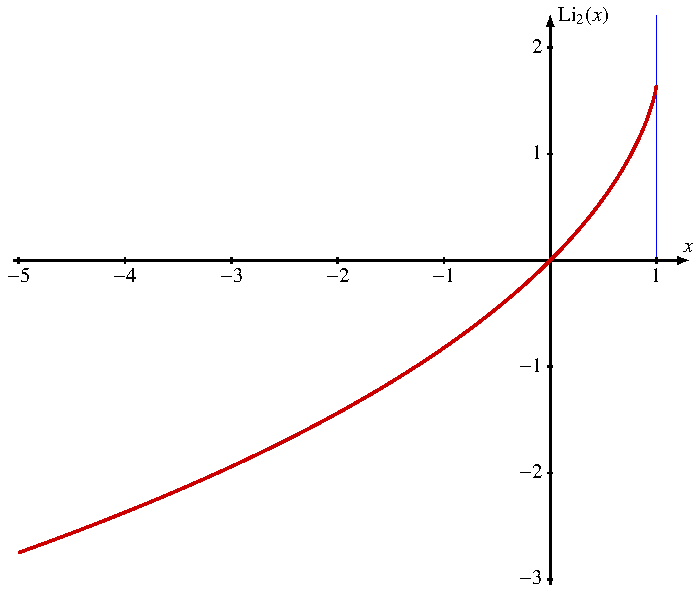
\includegraphics{chapters/070-intalg/images/li2.pdf}
\caption{Graph der Dilogarithmusfunktion
$\operatorname{Li}_2(x)$ für $x<1$.
\label{buch:intalg:fig:li2}}
\end{figure}
%
Aus der Ableitung~\eqref{buch:intalg:exp:dilog:integraldef}
folgt die Integraldefinition
\[
\operatorname{Li}_2(x)
=
-\int_0^x
\frac{\log(1-t)}{t}\,dt
\]
des Dilogarithmus für reelle Argumente $x\in(-\infty,0)$, die als
Basis für die graphische Darstellung des Graphen von
$\operatorname{Li}_2(x)$ 
in Abbildung~\ref{buch:intalg:fig:li2} diente.

Damit kann jetzt die Stammfunktion von $f(x)=x/(e^x+1)$ bestimmt werden.
Mathematica findet die Funktion
\index{Mathematica}%
\begin{align*}
F(x)
&=
-x\log(1+e^{-x})
+
\operatorname{Li}_2(-e^{-x}).
\intertext{Um davon die Ableitung zu berechnen, ist es nützlich, die
Ableitung von $\operatorname{Li}_2(-e^{-x})$ haben.
Sie ist}
\frac{d}{dx}
\operatorname{Li}_2(-e^{-x})
&=
\log(1+e^{-x}).
\intertext{Die Ableitung von $F(x)$ wird damit}
\frac{d}{dx}F(x)
&=
-\log(1+e^{-x})
-x\frac{1}{1+e^{-x}}\frac{d}{dx}(e^{-x})
+
\log(1+e^{-x})
\\
&=
-
\log(1+e^{-x})
+
x\frac{1}{1+e^{-x}}e^{-x}
+
\log(1+e^{-x})
\\
&=
x\frac{e^{-x}}{1+e^{-x}}.
\intertext{Erweitern mit $e^x$ ergibt}
&=
\frac{x}{e^x+1}.
\end{align*}
Damit ist gezeigt, dass $F(x)$ tatsächlich die Stammfunktion von $f(x)$
ist.

Das Computeralgebrasystem Maxima findet eine auf den ersten Blick gänzlich
andere Stammfunktion, nämlich
\begin{align}
G(x)
&=
\frac{x^2}2 - x \log(e^x+1) - \operatorname{Li}_2(-e^{x}).
\notag
\intertext{In diesem Fall brauchen wird die Ableitung}
\frac{d}{dx}\operatorname{Li}_2(-e^x)
&=
-\log(e^x+1).
\intertext{Die Ableitung von $G(x)$ wird damit}
\frac{d}{dx}G(x)
&=
x-\log(e^x+1) - \frac{xe^x}{e^x+1} 
+
\log(e^x+1)
\notag
\\
&=
\frac{x(e^x+1)-xe^x}{e^x+1} 
\notag
\\
&=
\frac{x}{e^x+1}.
\end{align}
Auch diese Form der Stammfunktion ist also korrekt.

Die beiden Stammfunktionen $F(x)$ und $G(x)$ können sich um höchstens
eine Konstante unterscheiden, die Differenz ist 
\begin{align}
C
=
F(x)-G(x)
&=
-x\log(1+e^{-x})+\operatorname{Li}_2(-e^{-x})
-\frac{x^2}2+x\log(e^x+1)+\operatorname{Li}_2(-e^x)
\notag
\intertext{Die Konstante kann durch Evaluieren für $x=0$ gefunden werden,
sie stellt sich als $C=0$ heraus.
Die beiden Logarithmus-Terme können als Logarithmus eines Bruchs
geschrieben werden:}
0
&=
-x\log\frac{1+e^{-x}}{e^x+1}+\operatorname{Li}_2(-e^{-x})
-\frac{x^2}2+\operatorname{Li}_2(-e^x)
\notag
\\
&=
-x\log e^{-x}
-
\frac{x^2}2
+
\operatorname{Li}_2(-e^{-x})
+
\operatorname{Li}_2(-e^x)
\notag
\\
0
&=
\frac{x^2}2
+
\operatorname{Li}_2(-e^{-x})
+
\operatorname{Li}_2(-e^x),
\label{buch:intalg:risch:li2identity}
\end{align}
eine nichttriviale Identität für den Dilogarithmus.

Die Ableitung von
$
\operatorname{Li}_2(-e^{-x})
+
\operatorname{Li}_2(-e^x)
$
ist
\begin{align*}
\frac{d}{dx}\Bigl(
\operatorname{Li}_2(-e^{-x})
+
\operatorname{Li}_2(-e^x)
\Bigr)
&=
\log(1+e^{-x})-\log(e^x+1)
\\
&=
\log\frac{1+e^{-x}}{e^x+1}
=
\log e^{-x}
=
-x
\end{align*}
mit der Stammfunktion $-\frac{x^2}{2}$, was 
\eqref{buch:intalg:risch:li2identity}
bestätigt.

%
% Der polynomielle Teil und die Risch-Differentialgleichung
%
\subsubsection{Der polynomielle Teil und die Risch-Differentialgleichung}
Der polynomielle Teil des Integranden $f\in F(\vartheta)$ ist eine 
erweitertes Polynom der Form
\[
p(\vartheta)
=
\sum_{i=-k}^l
p_i\vartheta^i,
\]
dessen Stammfunktion jetzt analog zum logarithmischen Fall durch
Koeffizientenvergleich ermittelt werden soll.

Die Ableitung eines Monoms ist
\[
D(a\vartheta^n) 
=
(Da)\vartheta^n + an\vartheta^{n-1}D\vartheta
=
(Da)\vartheta^n + an\vartheta^{n-1}\vartheta Du
=
(Da + naDu)\vartheta^n,
\]
also wieder ein Monom mit dem gleichen Exponenten.
Die Ableitung reduziert im Gegensatz zum logarithmischen Fall den
Grad nicht.
Man darf daher erwarten, dass die Stammfunktion wieder ein erweitertes
Polynom
\[
q(\vartheta)
=
\sum_{i=-k}^l q_i\vartheta^i
\]
ist.

Um die Koeffizienten des Polynoms zu finden, leiten wir $q(\vartheta)$
ab und führen Koeffizientenvergleich in
\[
p(\vartheta)
=
\sum_{i=-k}^l p_i\vartheta^i
=
Dq\vartheta
=
\sum_{i=-k}^l
(Dq_i + iq_i Du)\vartheta^i
\]
durch.
Es ergeben sich die Differentialgleichungen
\begin{equation}
Dq_i + iDu\cdot q_i = p_i
\label{buch:intalg:risch:exponentiell:eqn:rischdgl}
\end{equation}
für $i =-k,\dots, l$.
Gesucht sind Lösungen $q_i\in F$.
Falls es keine solche Lösung gibt, hat $p(\vartheta)$ keine elementare
Stammfunktion.

Auf den ersten Blick scheint es, dass die Differentialgleichung
\eqref{buch:intalg:risch:exponentiell:eqn:rischdgl}
das Integrationsproblem in eine Differentialgleichungsproblem
umwandelt.
Die Bestimmung einer Stammfunktion ist ein Spezialfall der Lösung
einer Differentialgleichung, man könnte also meinen, dass das
ursprüngliche Problem durch ein schwierigeres Problem ersetzt worden
ist.
Zudem sagen doch die bekannten Sätze aus der Theorie der gewöhnlichen
Differentialgleichungen, dass die Lösung mindestens lokal existiert
und eindeutig ist.
Es geht aber nicht darum, eine beliebige Lösungsfunktion zu finden,
sondern diese Funktion muss in $F$ sein.
Der Satz von Picard-Lindelöf als Beispiel eines Existenz- und
Eindeutigkeitssatzes für gewöhnliche Differentialgleichungen
kann dazu nichts aussagen.
Daher wurden auch gänzlich andere Methoden zur Lösung dieser
Differentialgleichung entwickelt.

\begin{definition}[Risch-Differentialgleichung]
Sei $F$ ein differentieller Funktionenkörper und $f,g\in F$.
Das Problem, eine Lösung $y\in F$ der Differentialgleichung
\[
Dy + f\, y = g
\]
zu finden, heisst die \emph{Risch-Differentialgleichung}.
\end{definition}

\begin{beispiel}
Hat die Wahrscheinlichkeitsdichte $e^{-x^2/2}$ eine elementare
Stammfunktion?
Der Integrand ist in der Erweiterung $F(\vartheta)=K(x,\vartheta)$
von $F=K(x)$ um die Exponentialfunktion $\vartheta = e^{-x^2/2}$
von $u=-x^2/2$.
Gesucht ist die Stammfunktion des polynomiellen Teils
$p(\vartheta)=p_1\vartheta^1$.
Sie muss die Form $q_1\vartheta$ haben.
Die Risch-Differentialgleichung ist
\[
Dq_1 + Du\, q_1 = p_1
\quad\Rightarrow\quad
Dq_1 - x q_1 = 1.
\]
Die Lösung muss eine rationale Funktion $q_1\in K(x)$ sein.
Wir schreiben die rationale Funktion als gekürzten Bruch
\begin{equation}
q_1(x) = \frac{a(x)}{b(x)}
\label{buch:intalg:risch:exponentiell:bsp:eqn:qex2}
\end{equation}
von Polynomen $a,b\in K[x]$, $b(x)$ soll ausserdem normiert sein.
Einsetzen in die Differentialgleichung liefert
\begin{align}
\frac{a'(x)b(x)-a(x)b(x)}{b(x)^2} - x\frac{a(x)}{b(x)} &= 1.
\notag
\intertext{Multiplizieren mit dem Nenner $b(x)^2$ führt auf die
Polynomgleichung}
a'(x)b(x) - a(x)b'(x) -x a(x)b(x) &= b(x)^2.
\label{buch:intalg:risch:exponentiell:eqn:qex2poly}
\end{align}
Das Polynom $b(x)$ ist ein Teiler des ersten und des letzten Terms auf
der linken Seite.
Ausserdem teilt es die rechte Seite.
Daher muss es auch den mittleren Term $a(x)b'(x)$ teilen.
Es kann aber keine gemeinsamen Faktoren mit $a(x)$ haben, da angenommen
wurde, dass der Bruch \eqref{buch:intalg:risch:exponentiell:bsp:eqn:qex2}
gekürzt ist.
Es folgt, dass $b(x)$ die Ableitung $b'(x)$ teilt, was nur möglich ist,
wenn $b'(x)=0$ ist.
Das Polynom $b(x)$ ist also nur ein Konstante $b_0$.
Da $b(x)$ ausserdem normiert ist, muss $b_0=1$ sein.

Die Polynomgleichung \eqref{buch:intalg:risch:exponentiell:eqn:qex2poly}
wird jetzt zu
\begin{equation}
a'(x) - x a(x) = 1.
\label{buch:intalg:risch:exponentiell:bsp:eqn:qex2:adgl}
\end{equation}
Schreibt man die Koeffizienten des Polynoms als $a_k$, wird die
Gleichung
\eqref{buch:intalg:risch:exponentiell:bsp:eqn:qex2:adgl}
zu
\begin{align*}
\sum_{k=0}^n ka_kx^{k-1} -x \sum_{k=0}^n a_kx^k &= 1
\\
\sum_{k=1}^n ka_kx^{k-1} - \sum_{k=0}^n a_kx^{k+1} &= 1
\\
\sum_{i=0}^{n-1} (i+1)a_{i+1}x^i - \sum_{i=1}^{n+1} a_{i-1} x^i &= 1
\\
a_1 + \sum_{i=1}^{n-1} \bigl((i+1)a_{i+1}-a_{i-1}\bigr) x^i
+ a_{n-1}x^n + a_{n}x^{n+1} &= 1
\end{align*}
Durch Koeffizientenvergleich liest man die Gleichungen
\begin{align}
a_1 &= 1 \notag \\
(i+1)a_{i+1} -a_{i-1} &= 0 &&\Rightarrow& a_{i-1} &= (i+1)a_{i+1}&&1\le i\le n-1
\label{buch:intalg:risch:exponentiell:bsp:exp2:rekursion}
\\
a_{n-1} &= 0 \notag \\
a_n &= 0 \notag
\end{align}
für die Koeffizienten $a_k$ ab.

Anwendung der Gleichung
\eqref{buch:intalg:risch:exponentiell:bsp:exp2:rekursion} auf
die letzten beiden Bedingungen erlaubt zu schliessen, dass alle
Koeffizienten verschwinden müssen, auch $a_0$.
Dies steht im Widerspruch zur ersten Gleichung $a_1=1$.
Der Widerspruch zeigt, dass die Lösung der Differentialgleichung
keine rationale Funktion sein kann und dass somit auch $e^{-x^2/2}$ keine
elementare Stammfunktion haben kann.
\end{beispiel}

%
% Anwendung: Integration der trigonometrischen Funktionen
%
\subsubsection{Anwendung: Integration der trigonometrischen Funktionen}
Die trigonemetrischen Funktion $\cos x$ und $\sin x$ liegen in der
exponentiellen Erweiterung $\mathbb{Q}(i,x,\vartheta)$ mit
$\vartheta=e^{ix}$.
Wie in Abschnitt \ref{buch:intalg:section:elementar} gezeigt wurde,
ist
\begin{align*}
\cos x
&=
\frac{\vartheta+1/\vartheta}{2}
=
\frac{\vartheta^2+ 1}{\vartheta}
=
\frac12\vartheta + \frac{1/2}{\vartheta}
\\
\sin x
&=
\frac{1}{2i}\vartheta
-
\frac{1/2i}{\vartheta}.
\end{align*}
Man beachte, dass beide Ausdrücke verallgemeinerte Polynome sind.
Zur Bestimmung der Stammfunktion von $\cos x$ sind also die
Risch-Differentialgleichungen
für das Polynom mit den Koeffiziente $p_1=\frac12$ und $p_{-1}=\frac12$
zu lösen:
\begin{align*}
Dq_{\pm 1} \pm i q_{\pm 1} = \frac12
\end{align*}
hat die konstante Lösung $q_{\pm 1} = \pm\frac{1}{2i}$.
Die Stammfunktion ist daher
\[
\int\cos x
=
q_1\vartheta + q_{-1}\frac{1}{\vartheta}
=
\frac{1}{2i}\biggl(\vartheta-\frac1{\vartheta}\biggr)
=
\sin x.
\]
Analog findet man auch die Stammfunktion von $\sin x$.
Der Algorithmus reproduziert also die bekannten Integrationsformeln für
die grundlegenden trigonometrischen Funktionen.

Für die Tangensfunktion gilt
\[
\tan x
=
-i
\frac{\vartheta-1/\vartheta}{\vartheta+1/\vartheta}
=
-i
\frac{\vartheta^2-1}{\vartheta^2+1}
=
-i
+\frac{2i}{\vartheta^2+1}.
\]
Auf den letzten Bruch kann die Methode von Rothstein-Trager angewendet
werden.
Es müssen gemeinsame Teiler von
\[
2i - ic\cdot 2\vartheta^2
=
2i(1-c\vartheta^2)
\qquad\text{und}\qquad
\vartheta^2+1
\]
gefunden werden.
Ein nichttrivialer gemeinsamer Teiler existiert für $c=-1$ und der grösste
gemeinsame Teiler ist $\vartheta^2+1$.
Somit ist
\[
\int \frac{2i}{\vartheta^2+1} = -\log(\vartheta^2+1)
\]
Es folgt, dass
\[
\int \tan x
=
-ix
-
\log(e^{2ix} + 1)
=
\log(e^{-ix})
-
\log(e^{2ix}+1)
=
\log\frac{e^{-ix}}{e^{2ix}+1}
=
\log\frac{1}{e^{ix}+e^{-ix}},
\]
was bis auf eine Konstante mit $\log(\sec(x))$ übereinstimmt.

